% Options for packages loaded elsewhere
\PassOptionsToPackage{unicode}{hyperref}
\PassOptionsToPackage{hyphens}{url}
%
\documentclass[
]{article}
\usepackage{amsmath,amssymb}
\usepackage{iftex}
\ifPDFTeX
  \usepackage[T1]{fontenc}
  \usepackage[utf8]{inputenc}
  \usepackage{textcomp} % provide euro and other symbols
\else % if luatex or xetex
  \usepackage{unicode-math} % this also loads fontspec
  \defaultfontfeatures{Scale=MatchLowercase}
  \defaultfontfeatures[\rmfamily]{Ligatures=TeX,Scale=1}
\fi
\usepackage{lmodern}
\ifPDFTeX\else
  % xetex/luatex font selection
\fi
% Use upquote if available, for straight quotes in verbatim environments
\IfFileExists{upquote.sty}{\usepackage{upquote}}{}
\IfFileExists{microtype.sty}{% use microtype if available
  \usepackage[]{microtype}
  \UseMicrotypeSet[protrusion]{basicmath} % disable protrusion for tt fonts
}{}
\makeatletter
\@ifundefined{KOMAClassName}{% if non-KOMA class
  \IfFileExists{parskip.sty}{%
    \usepackage{parskip}
  }{% else
    \setlength{\parindent}{0pt}
    \setlength{\parskip}{6pt plus 2pt minus 1pt}}
}{% if KOMA class
  \KOMAoptions{parskip=half}}
\makeatother
\usepackage{xcolor}
\usepackage[margin=1in]{geometry}
\usepackage{graphicx}
\makeatletter
\def\maxwidth{\ifdim\Gin@nat@width>\linewidth\linewidth\else\Gin@nat@width\fi}
\def\maxheight{\ifdim\Gin@nat@height>\textheight\textheight\else\Gin@nat@height\fi}
\makeatother
% Scale images if necessary, so that they will not overflow the page
% margins by default, and it is still possible to overwrite the defaults
% using explicit options in \includegraphics[width, height, ...]{}
\setkeys{Gin}{width=\maxwidth,height=\maxheight,keepaspectratio}
% Set default figure placement to htbp
\makeatletter
\def\fps@figure{htbp}
\makeatother
\setlength{\emergencystretch}{3em} % prevent overfull lines
\providecommand{\tightlist}{%
  \setlength{\itemsep}{0pt}\setlength{\parskip}{0pt}}
\setcounter{secnumdepth}{5}
\usepackage[german]{babel}
\usepackage{mathtools}
\usepackage{tikz}
\usepackage{pgf}
\usepackage{csquotes}
\AtBeginDocument{
\renewcommand{\maketitle}{}
}
\PassOptionsToPackage{a4paper,margin = 2.5cm}{geometry}
\usepackage{geometry}
\usepackage{float}
\usepackage{enumitem}
\newcommand{\bcenter}{\begin{center}}
\newcommand{\ecenter}{\end{center}}
\renewcommand{\contentsname}{Inhalt}
\usepackage{blindtext}
\usepackage[backend=biber, style = apa]{biblatex}
\addbibresource{Literatur.bib}
\usepackage{multirow}
\usepackage{booktabs}
\usepackage{array}
\usepackage{pdflscape}
\usepackage{afterpage}
\ifLuaTeX
  \usepackage{selnolig}  % disable illegal ligatures
\fi
\usepackage[]{biblatex}
\addbibresource{Literatur.bib}
\usepackage{bookmark}
\IfFileExists{xurl.sty}{\usepackage{xurl}}{} % add URL line breaks if available
\urlstyle{same}
\hypersetup{
  pdftitle={Hausarbeit},
  pdfauthor={Franz Andersch \& Niklas Münz},
  hidelinks,
  pdfcreator={LaTeX via pandoc}}

\title{Hausarbeit}
\author{Franz Andersch \& Niklas Münz}
\date{2024-08-29}

\begin{document}
\maketitle

\begin{titlepage}
	\begin{center}
		
		
\includegraphics[width=0.5\textwidth]{images/UB-Logo-blau.png}
		
		\LARGE
		\textbf{Otto-Friedrich Universität Bamberg}\\
		\textbf{Lehrstuhl für Statistik und Ökonometrie}\\
		\textbf{Statistical Machine Learning}
		
		
		\vspace*{1.5cm}
		
		\Huge
		\textbf{Unser Thema}
		
		
		\vspace{2cm}
		
		\Large
		\begin{minipage}[t]{0.4\textwidth}
			\textbf{Autoren:}
		\end{minipage}
		\hfill
		\begin{minipage}[t]{0.3\textwidth}
			Niklas Münz\newline
			Matrikel Nr.: 2150715
			
			\vspace{0.3cm}
			
			Franz Andersch\newline
			Matrikel Nr.: 2154877
			
		\end{minipage}
		
		\vspace{0.5cm}
		
		\Large
		\begin{minipage}[t]{0.4\textwidth}
			\textbf{Studiengang:}
		\end{minipage}
		\hfill
		\begin{minipage}[t]{0.3\textwidth}
			MSc. Survey Statistics \newline
			\& Data Analysis
		\end{minipage}
		
		\vfill
		Sommersemester 2024
		
	\end{center}
\end{titlepage}
\newpage
\tableofcontents
\thispagestyle{empty}
\clearpage
\pagenumbering{arabic}
\section{Einleitung}

Bei der Separierung von zwei Datenklassen scheint eine lineare
Trennlinie zwischen die Klassen zu ziehen eine simple und intuitive
Methode zu sein. Genau auf dieser Idee basieren Support Vector Machines
(SVM). Jedoch sind Daten nicht immer perfekt trennbar oder es liegt
keine lineare Trennlinie vor. Wie SVM funktionieren, wie sie mit solchen
Situationen umgehen, wie sie unter vorgegebenen Bedingungen performen
und welche Schlussfolgerungen für die praktische Anwendung gezogen
werden können, soll in dieser Arbeit beleuchtet werden.

Die Grundlage für eine optimal separierende Hyperebene wurde bereits
1964 von Alexej Chervonenkis und Vladimir Vapnik gelegt und die Methode
wurde anschließend von mehreren Autoren stetig erweitert
\parencite{vapnikEstimationDependencesBased2006}. Seitdem ist ihre
Leistung, trotz großer Fortschritte im Bereich neuronaler Netze, vor
allem im Bereich binärer Klassifikationsprobleme unumstritten und sie
gelten dabei als eine der meistgenutzten Methoden
\parencite{soofiClassificationTechniquesMachine2017}. Dabei bieten SVM
eine große Anzahl an Anwendungsmöglichkeiten, wie beispielsweise, in der
Bildklassifikation, in der Bioinformatik (Krebsklassifikation) oder im
Aufdecken von Kreditkartenbetrug
\parencite{cervantesComprehensiveSurveySupport2020}.

In dieser Arbeit wollen wir zuerst die Funktionsweise der SVM näher
betrachten. Dazu wird zunächst gezeigt wie die Konstruktion dieser
separierenden Hypereben im Falle linear trennbarer Daten funktioniert.
Daraufhin wird die Idee eines Soft Margin Classifier aufgegriffen, der
sich dem Problem nicht trennbarer Daten annimmt. Zuletzt geht es um die
Anwendung von Kernels, die es ermöglichen, nicht lineare
Entscheidungsgrenzen herzustellen.\newline In Kapitel 3 werden dann die
Vor- und Nachteile der Methode betrachtet. Anhand dieser Informationen
werden Schlussfolgerungen zur Leistung der SVM gezogen. Darauf aufbauend
wird im folgenden Kapitel der Aufbau unseres Experiments beschrieben.
Wir generieren uns zum anschließenden Vergleich neun verschiedene
Datenszenarien, welche in ihrer Dimensionalität und Komplexität der
Entscheidungsgrenze variieren. Für die Evaluierung der
Klassifikationsleistung werden neben den SVM weitere
Klassifikationsmethoden herangezogen.\newline Im Kapitel Hypothesen
wurden auf Basis von Literatur, in der bereits ähnliche Versuche
durchgeführt wurden, Vermutungen aufgestellt, wie die einzelnen
Klassifikationsmethoden im Vergleich abschneiden werden.\newline Es
folgen die Ergebnisse, in denen die Durchführung des Experiments
beschrieben und die Leistungen anhand verschiedener Maßzahlen evaluiert
werden. Darüber hinaus wird überprüft, ob sich die Hypothesen die wir
zuvor aufgestellt haben bewahrheitet haben. Im letzten Abschnitt wird
ein Fazit gezogen, indem die Ergebnisse diskutiert und
Weiterentwicklungsmöglichkeiten für unsere Arbeit aufgearbeitet werden.

\section{Funktionsweise}

\subsection{Hard Margin Classifier}

Um das grundlegende Prinzip der SVM darzustellen, gehen wir zuerst von
einer Datensituation aus, in der sich zwei Gruppen optimal durch eine
lineare Entscheidungsgrenze trennen lassen. Das endgültige Ziel ist es
eine sogenannte Hyperplane zu finden die diese Daten möglichst gut
separiert und als Entscheidungsgrenze funktioniert. Die allgemeine Form
einer solchen Hyperplane lautet \begin{align}
\beta_0+ \beta_1 X_1+\beta_2 X_2+...+\beta_n X_n=0\label{eq:hyperebene}
\end{align} oder in Vektorschreibweise \begin{align}
\overline{\beta}\cdot\overline{x}+\beta_0=0 \label{eq:hyperplanevec}
\end{align} Die geometrische Interpretation des Vektors \(\beta\) und
des Skalars \(\beta_0\) wird in Abbildung \ref{fig:Ebene} im
zweidimensionalen Fall dargestellt.

\begin{figure}[htb]
    \centering
    \begin{minipage}{0.45\textwidth} 
        \centering
        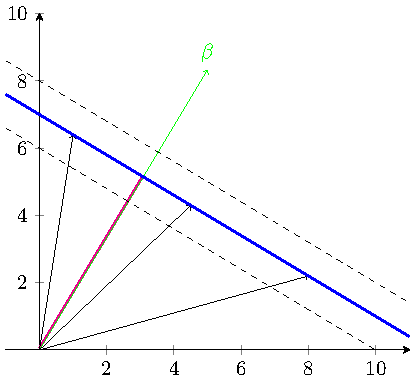
\includegraphics[width=\textwidth,trim=0.5cm 0.5cm 0.5cm 0.5cm]{Images/decision_boundary.pdf} 
        \caption{Konstruktion der Hyperebene}
        \label{fig:Ebene}
    \end{minipage}\hfill
    \begin{minipage}{0.45\textwidth} 
        \centering
        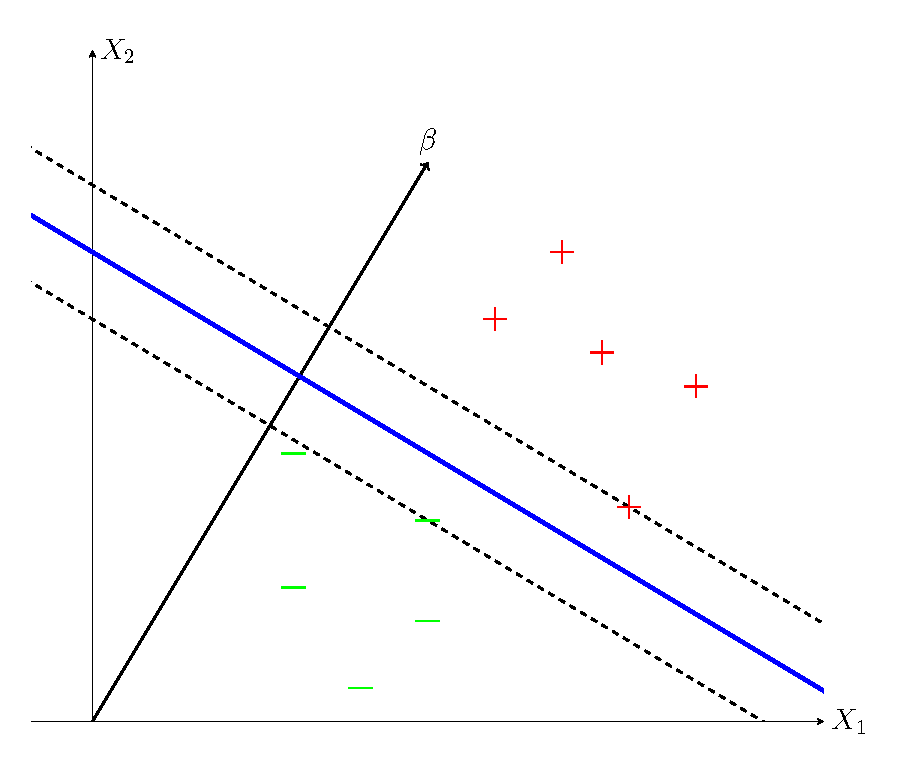
\includegraphics[width=\textwidth,trim=0.5cm 0.5cm 0.5cm 0.5cm]{Images/guttes.pdf}
        \caption{Konstruktion der Margins}
        \label{fig:Margin}
    \end{minipage}
\end{figure}

Die blaue Linie soll die Hyperplane darstellen. Im zweidimensionalen
handelt es sich hier um eine Linie. Der \(2 \times 1\) Vektor
\(\overline{\beta}\) liegt immer senkrecht zur konstruierten Hyperplane.
Würde man alle Vektoren, die auf der Hyperplane landen, auf den
normierten \(\overline{\beta}\)-Vektor projizieren, dann erhält man für
alle diese Projektionen denselben Wert \(c\). Also gilt für alle Punkte,
die auf der Ebene liegen. \begin{align}
\frac{\overline \beta}{||\overline{\beta}||}\cdot \overline{x}=c \Leftrightarrow \overline{\beta}\cdot \overline{x}=c \cdot ||\overline{\beta}||\label{eq:betanull}
\end{align} Ersetzt man in \eqref{eq:betanull}
\(c \cdot ||\overline{\beta}||\) mit \(-\beta_0\) und zieht dies dann
auf die andere Seite, kommt man wieder bei der ursprünglichen Form aus
Formel \eqref{eq:hyperplanevec} raus
\parencite{mavroforakisGeometricApproachSupport2006}.

Als Nächstes stellt sich jetzt die Frage, welches \(\overline{\beta}\)
und \(\beta_0\) die optimale Hyperplane darstellen. Betrachtet man die
Abbildung \ref{fig:Margin}, dann ist zu erkennen, dass die Datenpunkte
durch die blaue Linie getrennt werden. Allerdings könnte man theoretisch
unendlich viele andere Hyperplanes durch Rotation oder Verschiebung
konstruieren, die trotzdem die Daten in ihren Ausprägungen trennen. Um
eine eindeutige Lösung zu finden, wird zunächst ein Bereich um die
Hyperplane abgesteckt. In Abbildung \ref{fig:Margin} dargestellt durch
die gestrichelten schwarzen Linien, welche man als Schranken bezeichnen
könnte. In diesem Bereich sollen keine Datenpunkte liegen, die Schranken
sollen immer parallel zur Hyperplane sein und den gleichen Abstand zu
ihr haben. Außerdem dürfen keine positiven Samples unterhalb der oberen
Schranke liegen und keine negativen oberhalb. Das Gegenteil gilt
dementsprechend für die untere Schranke. Als Definition für die beiden
Schranken wird festgelegt \begin{align}
\overline{\beta}\cdot \overline{x}+\beta_0=1\label{eq:posSV}
\end{align} für die Schranke in Richtung der grünen Datenpunkte und
\begin{align}
\overline{\beta}\cdot \overline{x}+\beta_0=-1\label{eq:negSV}
\end{align} für die Schranke in Richtung der roten Datenpunkte. Aus
dieser Beschränkung für die Hyperplane können wir auch ableiten, dass
für die positiven Samples \(\overline{x}^+\) immer gilt
\(\overline{\beta}\cdot \overline{x}^++\beta_0\ge 1\) und für negative
Samples \(\overline{x}^-\) immer gilt
\(\overline{\beta}\cdot \overline{x}^-+\beta_0\le -1\). Durch das
Einführen einer weiteren Variable \(y\), welche die Eigenschaft hat,
dass sie den Wert 1 bei einem positiven und den Wert -1 bei einem
negativen Sample annimmt, können diese zwei Beschränkungen zu Einer
zusammengefasst werden \parencite{cortesSupportvectorNetworks1995}.
\begin{align}
y_i(\overline{\beta}\cdot \overline{x}_i+\beta_0)\ge 1\label{eq:Nebenbedingung}
\end{align} Da das Verfahren auch \textit{Maximal Margin Classifier}
gennant wird, gilt es jetzt noch eine Definition für den Margin also den
Abstand zwischen den zwei Schranken zu finden, der letztendlich
maximiert werden soll. Damit diese Schranken, maximal weit auseinander
liegen, muss es zwangsläufig Datenpunkte geben, die genau auf den
Schranken liegen. Diese Datenpunkte haben eine wichtige Rolle für die
Konstruktion des Margins. Es sind ausschließlich diese Datenpunkte, die
einen Einfluss auf die finalen Werte von \(\overline{\beta}\) und
\(\beta_0\) haben werden. Sie werden \textit{Support-Vektoren} genannt
und geben den SVM ihren Namen.

\begin{figure}[htb]
\centering
 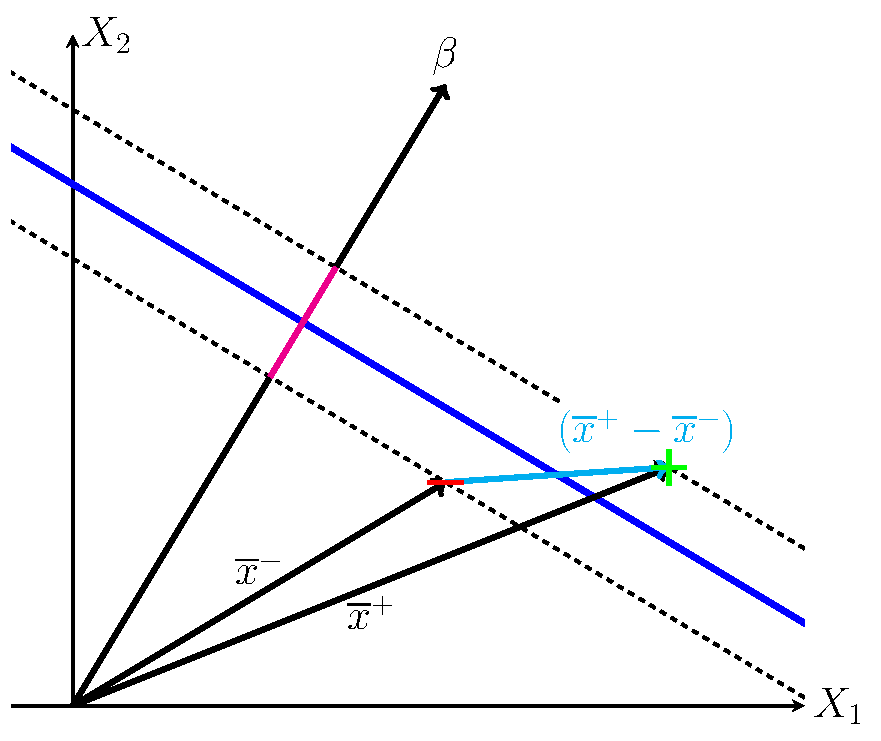
\includegraphics[width=0.5\textwidth,trim=0.5cm 0.5cm 0.5cm 0.5cm]{Images/margin.pdf} 
        \caption{Abhängigkeit des Margins von den Support-Vektoren}
        \label{fig:SupVecs}
\end{figure}

In Abbildung \ref{fig:SupVecs} sind zwei solcher Support-Vektoren zu
einem negativen und positiven Sample dargestellt. Der Margin kann dann
dargestellt werden als eine Projektion dieser Differenz
(\(\overline{x}^+-\overline{x}^+\)) auf den \(\overline{\beta}\)-Vektor.
Damit am Ende die Länge dieses Margins \(M\) herauskommt, muss
\(\overline{\beta}\) noch durch seine Länge geteilt werden.
\begin{align}
M=\frac{\overline{\beta}}{||\overline{\beta}||}\cdot \left(\overline{x}^+-\overline{x}^+\right)=\frac{\overline{\beta}\cdot\overline{x}^- -\overline{\beta}\cdot\overline{x}^+}{||\overline{\beta}||}\label{eq:maring1}
\end{align} Es ist bekannt, dass für positive Support-Vektoren gilt
\(\overline\beta \overline{x}^+ +\beta_0 = 1 \Leftrightarrow \overline\beta \overline{x}^+=1-\beta_0\)
und für negative
\(\overline\beta \overline{x}^- +\beta_0 = -1 \Leftrightarrow \overline\beta \overline{x}^-=-1-\beta_0\).
Setzt man dies ein in \eqref{eq:maring1}, erhält man als
Maximierungsziel \begin{align}
M=\frac{1-\beta_0-(-1-\beta_0)}{||\overline\beta||}=\frac{2}{||\overline\beta||}\label{eq:margin2}
\end{align} Um diesen Maximierungsschritt angenehmer zu gestalten, wird
an der Stelle versucht den Ausdruck
\(\frac{1}{2}||\overline \beta||^2=\frac{1}{2}\overline \beta '\cdot \overline \beta\)
zu minimieren. Was im Endeffekt ebenfalls dazu führt, dass der Ausdruck
in \eqref{eq:margin2} maximiert wird.

Dieses Optimierungsproblem mit der Nebenbedingung aus Formel
\eqref{eq:Nebenbedingung} lässt sich am besten über Lagrange-Multiplier
lösen \begin{align}
\mathcal{L}(\overline\beta,\beta_0,\overline \alpha)=\frac{1}{2}\overline \beta ' \overline \beta-\sum \alpha_i[y_i(\overline \beta \cdot \overline{x_i}+\beta_0)-1]\label{eq:Lagrange}
\end{align} wobei hier \(\overline{\beta}\) und \(\beta_0\) minimiert
und \(\overline{\alpha}\) maximiert wird
\parencite{vapnikEstimationDependencesBased2006}. Wird dieser Ausdruck
partiell abgeleitet und gleich null gesetzt erhält man als
Zwischenergebnis \begin{align}
\frac{\partial \mathcal{L}}{\partial \beta}=\beta-\sum \alpha_i y_i \overline{x_i}\overset{!}{=}0 \Rightarrow \beta=\sum \alpha_i y_i \overline{x_i}\label{eq:solutbeta}
\end{align} Somit zeigt sich, dass \(\overline{\beta}\) als
Linearkombination der Inputvektoren dargestellt werden kann. Weiterhin
gilt für \(\beta_0\) \begin{align}
\frac{\partial \mathcal{L}}{\partial \beta_0}=\sum \alpha_i y_i \overline{x_i}\overset{!}{=}0\label{eq:solutbeta0}
\end{align} Setzt man dies in \eqref{eq:Lagrange} ein erhält man einen
neuen Ausdruck, denn es gilt zu minimieren \begin{align}
\mathcal{L}(\overline \alpha)=-\frac{1}{2}\sum \sum \alpha_i \alpha_j y_i y_j \overline{x}_i \cdot \overline{x}_j+\sum \alpha_i\label{eq:dualproblem}
\end{align} Die Lösung für diesen Ausdruck erfolgt dann über sogenannte
\enquote{standard non linear optimization algorithms for quadratic forms}
\parencite{boserTrainingAlgorithmOptimal1992}. Nachdem für
\(\overline \alpha\) gelöst wurde, kann dies in \eqref{eq:solutbeta}
eingesetzt werden, um das optimale \(\overline{\beta}\) zu erhalten. Es
kann gezeigt werden, dass die gelösten \(\alpha_i\) lediglich für die
Support-Vektoren Werte ungleich Null annehmen. Somit ist der
Koeffizientenvektor \(\overline{\beta}\) sogar eine Linearkombination
von nur den Support-Vektoren
\parencite{boserTrainingAlgorithmOptimal1992}. Die letzte unbekannte
\(\beta_0\) kann gelöst werden, indem man mithilfe von einem
positiven/negativen Support Vektor \eqref{eq:posSV}/ \eqref{eq:negSV}
nach \(\beta_0\) löst.

Mit den gelösten Werten zur optimalen Hyperplane kann jetzt auch eine
Entscheidungsregel für ungelabelte Datenvektoren \(\overline{x}_u\)
konstruiert werden. Bedenkt man also, wenn man einen Vektor, der nicht
auf der Hypeplane liegt in \eqref{eq:betanull} einsetzt, erhält man also
\(\frac{\overline \beta}{||\overline{\beta}||}\cdot \overline{x}_u=c+k\).
Wenn \(k\) positiv ist, liegt der neue Datenpunkt oberhalb der
Hyperplane und wird somit als positives Sample gewertet. Wenn \(k\)
negativ ist, dann liegt der Datenpunkt unterhalb der Hyperplane und wird
als negativ gewertet. Mit der gleichen Umformung wie weiter oben schon
beschrieben kommt man zu einer Entscheidungsfunktion
\(f(\overline{x}_u)\) und einer daraus resultierenden Stufenfunktion
\(g(\overline{x}_u)\), die dann die Kategorisierung der neuen
Beobachtung vornimmt. \begin{align}
g(\overline{x}_u)=\begin{cases}\mathrm{positiv}&\text{wenn } f(\overline{x}_u)=\overline{\beta}\cdot \overline{x}_u+\beta_0 > 0\\
\mathrm{negativ} & \text{wenn }f(\overline{x}_u)=\overline{\beta}\cdot \overline{x}_u+\beta_0<0
\end{cases}\label{eq:decisionf}
\end{align}

\subsection{Soft Margin Classifier}

Dass die Daten sich perfekt linear trennen lassen ist zwar praktisch, um
die Vorgehensweise zu veranschaulichen, tritt aber in realen Situationen
so gut wie nie auf. Falls sich positive und negative Samples im Raum
überlappen, ist die Konstruktion einer Hyperplane wie beim
\textit{Hard Margin Classifier} unmöglich. Man müsste also entweder auf
eine nicht lineare Hyperplane ausweichen oder man weicht die Vorgaben
für die Konstruktion der Hyperplane etwas auf. Zweiteres ist genau das,
was durch die \textit{Soft Margin Classifier} erreicht wird. Die Vorgabe
für die Konstruktion der Schranken ermöglicht es, einzelnen Datenpunkten
auf der falschen Seite der Schranke, ja sogar der Entscheidungsgrenzen
zu liegen. Dafür wird für die Einschränkungen eine sogenannte
\textit{Slack-Variable} \(\varepsilon\) eingeführt
\parencite{jamesIntroductionStatisticalLearning2021}. Wie diese sich
auswirkt, ist in Abbildung \ref{fig:slackvariable} aufgeführt. Setzt man
diese in \eqref{eq:Nebenbedingung} ein, lautet die neue Nebenbedingung
\begin{align}
y_i(\beta \cdot \overline{x}_i-\beta_0)>1- \varepsilon_i \label{eq:nebbedsfm}
\end{align}

\begin{figure}[htb]
\centering
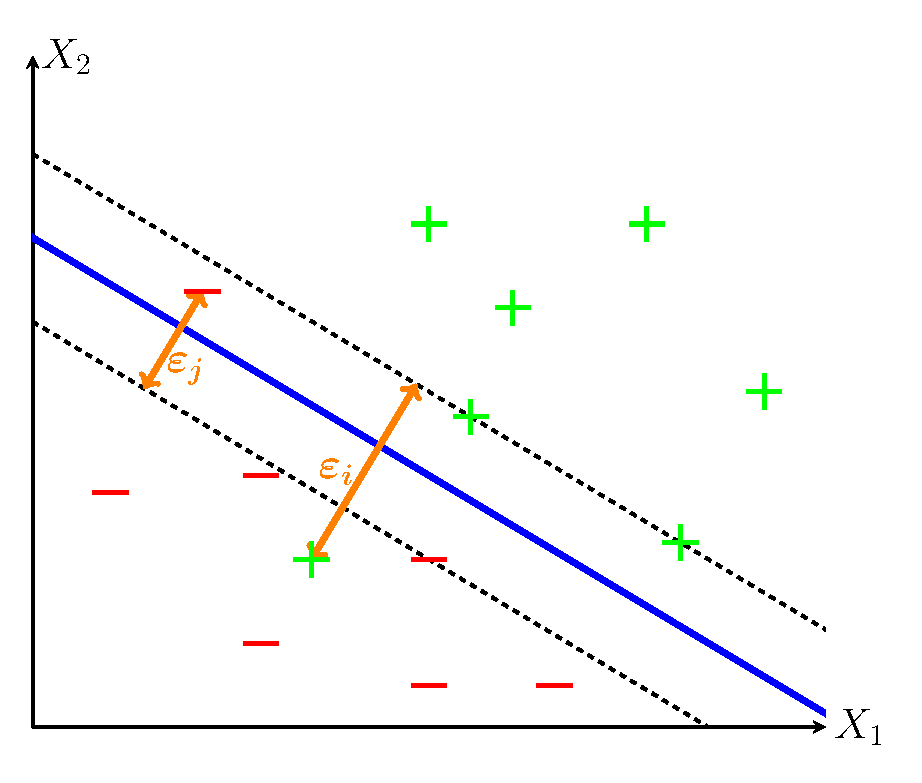
\includegraphics[width=0.5\textwidth,trim=0.5cm 0.5cm 0.5cm 0.5cm]{Images/slackvariable.pdf} 
        \caption{Bedeutung der Slack Variable}
        \label{fig:slackvariable}
\end{figure}

Jetzt könnte man versuchen, diese neue Nebenbedingung einfach in das
zuvor angewandte Optimierungsverfahren einzufügen. Allerdings besteht
hier das Problem, dass \(\varepsilon\) einfach immer maximal groß
gewählt wird und so die Bedingung immer erfüllt wird. Um das Ausmaß der
Verletzung der ursprünglichen Annahmen zu begrenzen, aber trotzdem noch
gewisse Abweichung zuzulassen, wird ein weiterer Parameter \(C\), als
regularisierender Parameter für \(\varepsilon\) eingeführt. Leitet man
daraus zusammen mit der Restriktion \(\varepsilon\ge0\) wieder eine
Lagrangefunktion her erhält man \begin{align}
\mathcal{L}(\overline\beta,\beta_0,\overline\alpha,\overline\varepsilon,\overline\lambda)=\frac{1}{2}\overline\beta'\cdot \overline\beta + C \sum_{i=1}^{n}\varepsilon_i-\underbrace{\sum \alpha_i[y_i(\overline\beta \cdot \overline{x_i}+\beta_0)-1+\varepsilon_i]}_{\text{für }y_i(\overline\beta \cdot \overline{x}_i-\beta_0)>1- \varepsilon_i}-\underbrace{\sum \lambda_i \varepsilon_i }_{\substack{\text{für}\\ \varepsilon_i \ge 0}}
\end{align} Wenn dieser Ausdruck wie beim
\textit{Hard Margin Classifier} gelöst wird und die Ergebnisse
eingesetzt werden erhält man wieder den Ausdruck aus
\eqref{eq:dualproblem} mit der zusätzlichen Einschränkung
\(0\le \alpha_i \le C\) \parencite{bennettSupportVectorMachines2000}.
Diese Min-Max-Optimierung wird dann genauso aufgelöst wie bei dem
\textit{Hard Margin Classifier} und die Entscheidungsregel ist ebenfalls
gleich. Erst durch den Einsatz dieser Technik wurde von der Methode auch
wirklich als \textit{Support Vector Machine} gesprochen
\parencite{vapnikEstimationDependencesBased2006}.

\subsection{Der Kernel Trick}

Auch wenn eine lineare Entscheidungsgrenze Vorteile in Sachen
Generalisierbarkeit bietet, ist sie doch nicht für jede Datensituation
geeignet.In Abbildung \ref{fig:nonlinearsep} ist es sehr gut zu
erkennen, dass in diesem Fall eine lineare Grenze zwischen den Klassen
keinen Sinn ergeben würde und eine elliptische Form wahrscheinlich
besser geeignet wäre. Eine Lösung für dieses Problem, wäre den
Merkmalsraum zu erweitern. So könnte die angenommene Formel für die
lineare Hyperebene in \eqref{eq:hyperebene} durch Polynome der Merkmale
\(X_i\) oder durch Interaktionsterme erweitert werden. Dies führt dazu,
dass die Entscheidungsgrenze in diesem vergrößerten Merkmalsraum immer
noch linear ist, aber die Trennung möglich ist (siehe Abbildung
\ref{fig:featurexten}). Transformiert man diese dann wieder in den
ursprünglichen Merkmalsraum ist die Entscheidungsgrenze dann nicht mehr
linear. Allerdings führt diese Herangehensweise zu einem starken Anstieg
des Rechenaufwands, da die Möglichkeiten der Merkmalserweiterung endlos
sind \parencite{jamesIntroductionStatisticalLearning2021}.

Die Lösung für das Problem sind sogenannte Kernel Funktionen. Betrachtet
man die Entscheidungsfunktion \eqref{eq:decisionf} und setzt für
\(\overline{\beta}\) die Gleichung aus \eqref{eq:solutbeta} erhält man
\begin{align}
f(x_u)= \sum \alpha_i y_i x_i \cdot x_u +\beta_0
\end{align} Es zeigt sich also, dass sich die Entscheidungsfunktion im
Wesentlichen aus einer Linearkombination von Punktprodukten aus dem
Vektor \(x_u\) mit allen Trainingsvektoren \(x_i\) ergibt. Dieses
Punktprodukt kann als Ähnlichkeitsmaß zwischen dem neuen Datenpunkt und
dem jeweiligen Trainingsdatenpunkt interpretiert werden. Es ist nun
möglich diese Produkte durch eine Funktion zu ersetzen, welche die
Ähnlichkeiten von Datenpunkten anders bewertet. Diese sogenannte
\textit{Kernel Funktion} \(K(x_i,x_j)\) ermöglicht es eine flexiblere
Entscheidungsgrenze zu implementieren. Der Vorteil ist dabei, dass die
Kernel Funktion nur auf alle Punktprodukte angewendet wird und es dabei
nicht nötig ist den Merkmalsraum zu erweitern, was wiederum Rechenzeit
spart \parencite{jamesIntroductionStatisticalLearning2021}. Die
Entscheidungsfunktion wird dann mithilfe dieser
\textit{Kernel Funktionen} berechnet: \begin{align}
  f(x_u)=\sum \alpha_i y_i K(x_i,x_u)+\beta_0
\end{align}

\begin{figure}[htb]
    \centering
    \begin{minipage}{0.45\textwidth} 
        \centering
        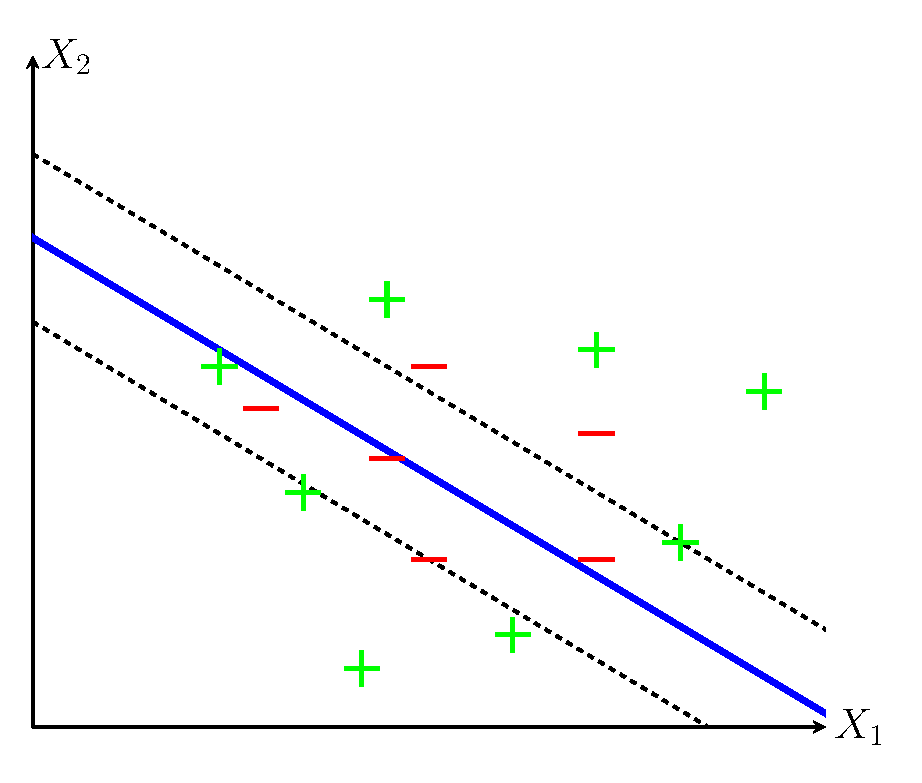
\includegraphics[width=\textwidth,trim=0.5cm 0.5cm 0.5cm 0.5cm]{Images/nonlinearseperable.pdf} 
        \caption{nicht linear getrennte Daten}
        \label{fig:nonlinearsep}
    \end{minipage}\hfill
    \begin{minipage}{0.45\textwidth} 
        \centering
        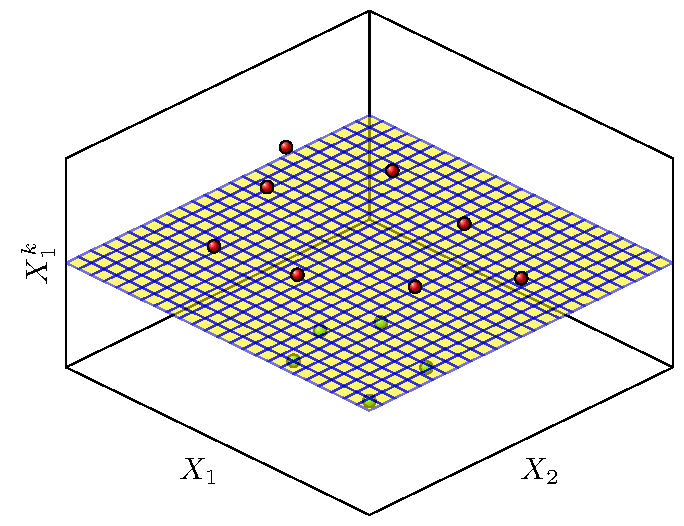
\includegraphics[width=\textwidth,trim=0.5cm 0.5cm 0.5cm 0.5cm]{Images/featurexpansion.pdf}
        \caption{Feature Erweiterung}
        \label{fig:featurexten}
    \end{minipage}
\end{figure}

Es gibt eine ganze Reihe an \textit{Kernel Funktionen}, die bei SVM
Anwendung finden. Die Grundlage ist der lineare Kernel, wobei dieser
lediglich das Punktprodukt beschreibt, also praktisch genau das macht,
was bei einer linearen Entscheidungsgrenze gemacht wird. Des Weiteren
gibt es den \textit{Polynomial Kernel}. Dieser hat die Form
\begin{align}
 K(x_i,x_u)=(1+x_i\cdot x_u)^d
\end{align} Die Verwendung von diesem Kernel führt dazu, dass die
Entscheidungsgrenze sich ähnlich Verhält, wie als würde man zu Beginn
eine Merkmalserweiterung mit Polynomen vom Grad \(d\) durchführen (siehe
Abbildung \ref{fig:polykernel}. Eine weitere Kernel Funktion ist der
\textit{Radial Basis Function Kernel} (RBF) mit der Form \begin{align}
K(x_i,x_u)=\exp\left(-\gamma ||x_i-x_u||^2\right)
\end{align} Für diesen Kernel wird die quadrierte euklidische Distanz
als Ähnlichkeitsmaß verwendet, was dazu führt, dass diejenigen \(x_i\)
die näher an \(x_u\) liegen, in der Entscheidungsfunktion einen größeren
Einfluss haben. Der Parameter \(\gamma\) legt dann fest, wie stark der
Einfluss der Distanz sein soll. Die Projektion die der Kernel hier macht
ist eine, in einen unendlich großen Merkmalsraum
\parencite{jamesIntroductionStatisticalLearning2021}. Daher könnte man
selbst durch vorheriges Erweitern des Merkmalsraums nicht das Ergebnis
eines RBF Kernel replizieren, daher führt er auch zu einer sehr
flexiblen Entscheidungsgrenze (siehe Abbildung
\ref{fig:radialkernel}).\\

\begin{figure}[htb]
    \centering
    \begin{minipage}{0.45\textwidth} 
        \centering
        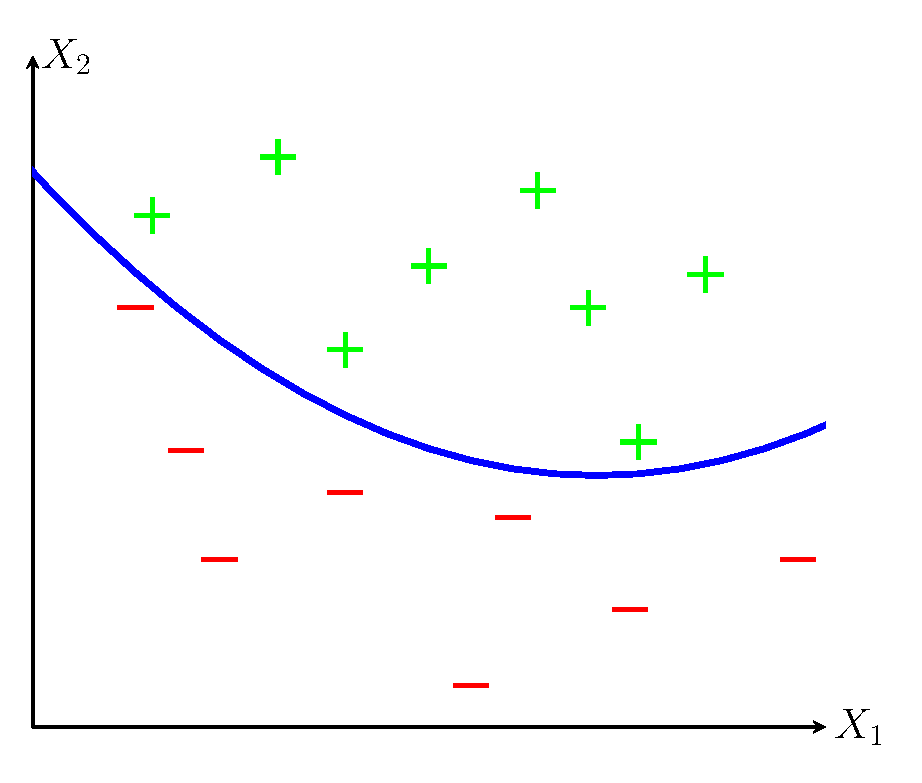
\includegraphics[width=\textwidth,trim=0.5cm 0.5cm 0.5cm 0.5cm]{Images/ploynomial kernel.pdf} 
        \caption{Mögliche Entscheidungsgrenze für polynomial Kernel}
        \label{fig:polykernel}
    \end{minipage}\hfill
    \begin{minipage}{0.45\textwidth} 
        \centering
        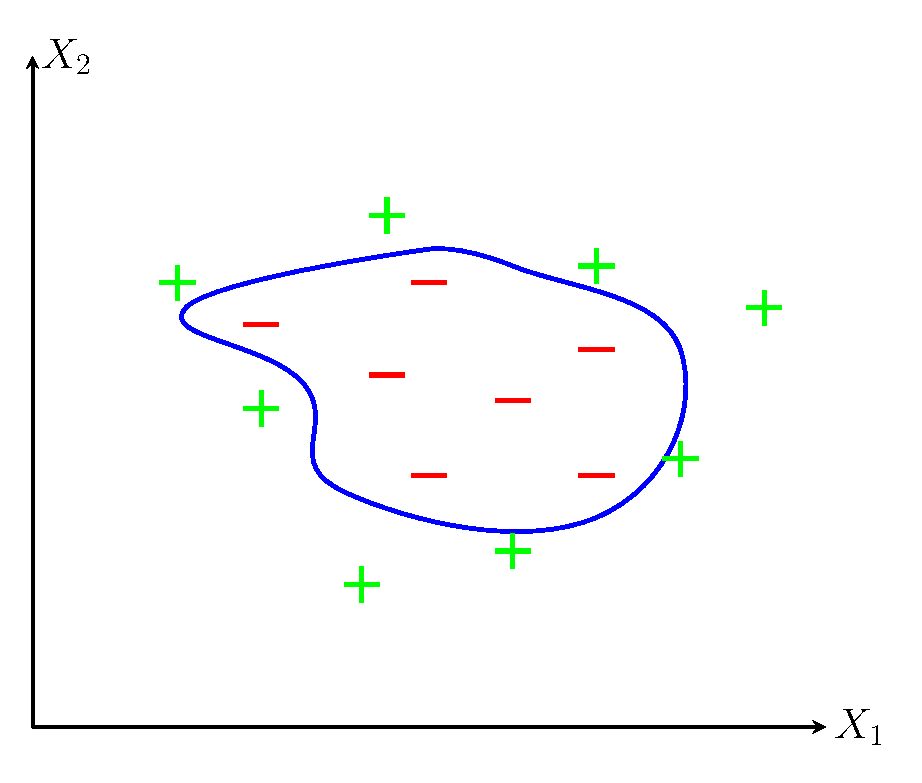
\includegraphics[width=\textwidth,trim=0.5cm 0.5cm 0.5cm 0.5cm]{Images/radial_kernel.pdf}
        \caption{Mögliche Entscheidungsgrenze für RBF Kernel}
        \label{fig:radialkernel}
    \end{minipage}
\end{figure}

Es gibt noch einen Reihe weitere Kernel, die auf unterschiedlichen
Ähnlichkeitsmaßen beruhen, aber eher seltener oder nur in speziellen
Zusammenhänge angewendet werden. Wichtig ist anzumerken, dass die
Verwendung von Kernels zwar die Flexibilität der Entscheidungsgrenze
erhöht, damit aber auch die Gefahr von \textit{Overfitting} einhergeht.
Zusätzlich werden mit den Kernels auch neue Hyperparameter wie \(d\)
oder \(\gamma\) eingeführt, die bei der Modellauswahl ebenfalls beachtet
werden müssen.

\section{Vor- und Nachteile der Methode}

Support Vector Machines haben ein hohes Ansehen unter den Machine
Learning Algorithmen, da sie einige Vorteile mit sich bringen. Aufgrund
der Idee einer Soft Margin und des ``Kernel Tricks'' ist die Methode
sehr flexibel und kann für spezielle Anwendungsbereiche angepasst werden
\parencite{bennettSupportVectorMachines2000}. Dazu sind die Ergebnisse
stabil und reproduzierbar, was sie von anderen Methoden wie
beispielsweise Neural Networks abhebt. Auch die Anwendung ist
vergleichsweise einfach, da es eine überschaubare Anzahl an Parametern
gibt (wie beispielsweise bei der \textit{SVM} mit radialem Kern nur der
gamma- und cost-Parameter festzulegen ist).\newline Durch die
Möglichkeit der Nutzung verschiedener Kerne sind \textit{SVM} überaus
vielseitig. Die Auswahl des Kerns ermöglicht es äußerst flexible
Entscheidungsgrenzen zu formen
\parencite{kuhnAppliedPredictiveModeling2013}. Dadurch können
\textit{SVM} an verschiedene Datensituationen angepasst werden.\newline
Ein weiterer Vorteil ist, dass die Methode weitgehend robust gegenüber
overfitting ist \parencite{kuhnAppliedPredictiveModeling2013}. Dafür
verantwortlich ist der Cost-Parameter, anhand dessen der Fit an die
Daten kontrolliert werden kann. Jedoch birgt dies auch Probleme
(Erläuterungen im folgenden Abschnitt).\newline Diese Vorteile
resultieren in einer allgemein häufigen Nutzung von \textit{SVM} in der
Wissenschaft, wobei sie schon oft bewiesen haben, dass sie für
verschiedenste Aufgaben gut funktionieren
\parencite{kuhnAppliedPredictiveModeling2013}.

Trotz der vielfachen Nutzung von \textit{SVM}, bringen sie auch
Nachteile mit sich. Das wohl größte Problem liegt in der Modellselektion
\parencite{bennettSupportVectorMachines2000}. Wie bereits im vorherigen
Abschnitt erwähnt, ist die Auswahl der Parameter von hoher Bedeutung bei
der Performance und dem Fit an die Daten. So kontrollieren die
Kernel-spezifischen Parameter und der Cost-Parameter einerseits die
Komplexität und andererseits den Fit an die Daten
\parencite{kuhnAppliedPredictiveModeling2013}. Dabei kann die Wahl der
Parameter sowohl zu einem Underfit als auch zu einem Overfit führen.
Jedoch haben nicht nur die Parameter einen Einfluss auf die Performance
sondern bereits die Wahl des Kernels kann entscheidend sein
\parencite{burgesTutorialSupportVector1998}. Je nach Datensituation
können SVM mit verschiedenen Kernels äußerst unterschiedliche Ergebnisse
liefern. Dies zeigt die Sensibilität der Methode gegenüber der Wahl des
Kerns und der Parameterabstimmung.\newline Ein weiterer Nachteil ist,
dass die Methode weniger intuitiv und aufwendiger anzuwenden ist als
andere Algorithmen \parencite{bennettSupportVectorMachines2000}. So ist
es zum Beispiel schwer Informationen aus Support Vektoren zu ziehen und
es gibt keine Koeffizienten die interpretiert werden können.\newline
Zuletzt ist zu erwähnen, dass die Methode bei einer hohen Anzahl an
Beobachtungen besonders rechenintensiv ist. So konnte beispielsweise
gezeigt werden, dass insbesondere die \textit{SVM} mit polynomialem und
radialem Kern eine hohe Rechenzeit aufweisen
\parencite{scholzComparisonClassificationMethods2021}. Dabei konnten
andere Methoden wie die \textit{logistische Regression} oder
\textit{k-nearest Neighbour} deutlich besser abschneiden. Dies liegt
daran, dass die Lösung des \textit{SVM}-Optimierungsproblems, die
Behebung eines quadratischen Programmierungsproblems erfordert. Da die
Anzahl der zu optimierenden Parameter mit der Anzahl der Daten
quadratisch zunimmt, führt dies zu einer hohen Rechenkomplexität
\parencite{kecmanSupportVectorMachines2005}.

\section{Daten}

Das Ziel dieser Arbeit ist es, in verschiedenen Datensituationen die
Performance von SVM Algorithmen für die binäre Klassifikation zu
evaluieren. Dafür wollen wir eine Reihe von Datensätzen mit
verschiedenen Charakteristiken synthetisch erstellen und entsprechend
als Trainingsdaten verwenden. Die Datensätze unterscheiden sich in zwei
zentralen Eigenschaften. Das erste sind die Dimensionen. Es soll
unterschieden werden in drei Kategorien. Die erste ist, dass es deutlich
mehr Beobachtungen als Variablen gibt, also \(n \gg p\). Ein solches
Datenszenario kann z.B. im Kontext des Zensus auftreten, in dem eine
große Anzahl an Personen befragt wird, aber die Vorgabe besteht, dass
die Bürger nicht zu stark belastet werden sollen, weshalb nur einige
wenige Kernfragen gestellt werden. In diesem Fall wurde für \(n=1000\)
Beobachtungen und \(p=10\) Variablen generiert. Das zweite Szenario
stellt Datensätze vor die etwa gleich viele Beobachtung wie Variablen
haben \(n \approx p\). Ein solches Szenario kann in vielen Kontexten
auftreten. Für dieses Szenario sind die Dimensionen \(n=p=50\). Das
letzte Szenario behandelt dann entsprechend den Fall \(n \ll p\). Dies
tritt oft im Kontext von Datenerhebungen im medizinischen Bereich auf,
da sehr viele Erhebungen zu kostspielig wären. Auch im Bereich des
Natural Language Processing sind solche Datensätze häufiger anzutreffen
\parencite{scholzComparisonClassificationMethods2021}. Die Werte die
dafür angenommen wurden sind \(p=200\) und \(n=50\).

Die zweite Charakteristik ist der Datengenerierende Prozess. Da in
dieser Arbeit SVM im Vordergrund stehen und wir hier vor allem zeigen
wollen, wie SVM funktionieren, wird der DGP so aufgebaut, dass er der
grundlegenden Idee der SVM am ehesten entspricht. Die Vorgehensweise
ist, im ersten Schritt eine Hyperplane, im \(p\)-Dimensionalen Raum, in
einer bestimmte Form zu erstellen und anschließend auf jeweils einer
Seite dieser Hyperplane \(n/2\) zufällige Punkte zu samplen, die die
jeweilige Ausprägung in der Zielvariable repräsentieren. Wir haben also
für die Zielvariable eine 50/50 Verteilung für die binären Ausprägungen
angenommen.

Insgesamt gibt es auch hier wieder 3 Kategorien. Die erste sind linear
getrennte Daten. Dafür wird eine lineare Hyperplane der Form
\begin{align*}
\beta_1 X_1+\beta_2 X_2 +...+\beta_{1-p} = \beta_p X_p
\end{align*} mit zufälligen Koeffizienten erzeugt. Diese Daten sollen
also den Annahmen entsprechend, die für SVMs mit linearem Kernel gelten.
Nachem für eine Beobachtung \(j\) zufällig ein Punkt auf der Ebene
gesampelt wurde, wurde dieser anschließend verschoben. Die Verschiebung
erfolgte über eine Skalierung des normierten Normalenvektors
\(k\left(\frac{\overline{\beta}}{||\overline{\beta}||}\right)\). \(k\)
ist dabei eine normalverteilte Zufallszahl mit Mittelwert \(\mu_k\) und
Varianz \(\sigma^2_k\). Dieser Prozess wird \(n/2\) mal wiederholt für
die eine Ausprägung der Zielvariable (\(y_i=1\)) und dementsprechend
\(n/2\) mal für die andere Ausprägung (\(y_i=-1\)), dann aber mit
\(-\mu_k\) als Mittelwert für \(k\). \newline In der zweiten Situation
hat die Hyperplane eine quadratische Form: \begin{align*}
\beta_0+\beta_1 X_1 + \beta_2 X_1^2+\beta_3 X_2+\beta_4 X_2^2+...+\beta_{2p-2}X_{p-1}+\beta_{2p-1}X_{p-1}^2=\beta_{2p} X_p
\end{align*} diese Form der Trennung stellt also eine
Merkmalserweiterung um quadratische Terme dar und funktioniert damit
ähnlich wie eine SVM mit polynomialen Kernel mit \(d=2\). Die
Verschiebung erfolgte hier nur durch Skalierung der Werte von \(X_p\)
ebenfalls mit \(k\sim\mathcal{N}(\mu_k,\sigma^2_k)\) für die eine
Ausprägung und \(k\sim\mathcal{N}(-\mu_k,\sigma^2)\) für die andere
Ausprägung.\newline  Der letzte DGP geht von einer noch komplexeren
Entscheidungsgrenzen aus. Es wird hier ein Hypershpäre im \(p\)
dimensionalen Raum erstellt und einmal innerhalb und einmal außerhalb
dieser gesampelt. Dafür wurde für eine Beobachtung \(j\), \(p-1\) Winkel
\(\theta\) zufällig erstellt, ein Radius \(r\) festgelegt und
anschließend die einzelnen Werte \(X_{1,j},X_{2,j},...,X_{p,j}\)
berechnet. Die Berechnung erfolgt dabei über die Definition von
sphärischen Koordinaten: \begin{align*}
        X_{1,j} &= r \cos(\theta_1)\\
        X_{2,j} &= r \sin(\theta_1)\cos(\theta_2)\\
        X_{3,j} &= r \sin(\theta_1)\sin(\theta_2)\cos(\theta_3)\\
        &\quad \vdots\\
        X_{p-1,j}&=r \sin(\theta_1)\ldots \sin(\theta_{p-2})\cos(\theta_{p-1})\\
        X_{p,j}&=r \sin(\theta_1)\ldots \sin(\theta_{p-2})\sin(\theta_{p-1})
    \end{align*} Dieser Vorgang wird dann \(n/2\) mal, wiederholt und
anschließend erfolgt die Verschiebung durch eine Skalierung des
jeweiligen normalisierten Datenvektors
\(k\left(\frac{\overline{x}}{||x||}\right)\). \(k\) ist auch hier wieder
eine Zufallsvariable mit \(\mu_k\) für die eine Ausprägung der
Zielvariable und \(-\mu_k\) für die andere Ausprägung. Die Streuung
bleibt bei beiden bei einem konstanten Wert \(\sigma^2_k\). Je nachdem
wie \(\mu_k\) und \(\sigma^2_r\) gewählt werden kann die Trennbarkeit
der Daten angepasst werden. Für alle Szenarien wurde ein Wert für
\(\mu_k\) und \(\sigma^2_k\) festgelegt, der für eine moderate
Überschneidung der zwei Klassen sorgt. Allerdings musste der Abstand in
den höherdimensionalen Szenarien etwas erhöht werden, da sonst die
Performance für alle Classifier sehr schlecht und damit nicht
vergleichbar war.

Es ergeben sich daher 9 unterschiedliche Datensituationen, welche in
ihren Dimensionen und Komplexität der Entscheidungsgrenze variieren. Die
Kürzel für die Situationen sind in Tabelle \ref{tab:datensituationen}
abgetragen

\begin{table}[H]
\begin{center}
\begin{tabular}{ |c|c|c|c| }
 \hline
  & linear & polynomial & radial \\
 \hline
 $p \ll n$ & S1 & S2 & S3 \\
 \hline
 $p \approx n$ & S4 & S5 & S6 \\
 \hline
 $p \gg n$ & S7 & S8 & S9 \\
 \hline
\end{tabular}
\end{center}
\caption{Datenszenarien}
\label{tab:datensituationen}
\end{table}

Zusätzlich soll nicht nur ein Vergleich zwischen der Performance der SVM
mit verschiedenen Kernels gemacht werden, sondern auch die Unterschiede
in der Klassifikationsgüte der SVM zu anderen gängigen
Klassifikationsmethoden gezeigt werden. Dafür werden regularized
Logistic Regression und k-nearest Neighbour als Vergleichsalgorithmen
hinzugezogen.

\section{Hypothesen}

Im Folgenden werden Studien hinzugezogen, um eine Einschätzung der
Performance in den verschiedenen Szenarien vorzunehmen und Hypothesen
abzuleiten. Vorab ist zu erwähnen, dass die Evaluation von
Klassifikationsmethoden anhand synthetischer Datensätze in der Literatur
begrenzt ist. Da für diese Arbeit die Form der Entscheidungsgrenze
entscheidend ist, werden dennoch ausschließlich Arbeiten mit
synthetischen Datensätzen zu Rate gezogen.\newline Aufgrund dessen, dass
der datengenerierende Prozess hier so ausgearbeitet wurde, dass er mit
den Annahmen der SVM arbeitet, erwarten wir zuerst einmal eine
durchschnittlich bessere Performance der SVM Classifier im Vergleich zu
den anderen Methoden.

\begin{minipage}{0.9\linewidth}
\begin{itemize}[leftmargin=0.1\linewidth]
\item[\textbf{H1:}] Die SVM-Classifier Performen über alle Datensituationen im Durchschnitt besser als die anderen Classifier.
\end{itemize}
\end{minipage}

Des Weiteren wurden in den einzelnen Kategorien des datengenerierenden
Prozesses die Entscheidungsgrenzen speziell auf verschiedene Kernels
zugeschnitten. Daher sollten SVM mit linearem Kernel im Setting mit
linearer Entscheidungsgrenze mindestens so gut oder besser als die
restlichen Classifier performen. Gleiches gilt für SVM mit polynomialen
Kernel im Setting mit einer quadratischen Entscheidungsgrenze und
radiale Kernel bei einer Hypershäre als Entscheidungsgrenze.

\begin{minipage}{0.9\linewidth}
\begin{itemize}[leftmargin=0.1\linewidth]
\item[\textbf{H2:}] Die SVM-Classifier mit dem Kernel, der für den jeweiligen DGP zugeschnitten ist sollten mindestens genauso gut oder besser performen als die restlichen Classifier.
\end{itemize}
\end{minipage}

Es konnte weiterhin gezeigt werden, dass in einem Szenario, indem
erheblich mehr Beobachtungen als Dimensionen und eine lineare
Entscheidungsgrenze vorliegen (S1), deutliche Unterschiede zwischen
\textit{SVM}, \textit{K-NN} und \textit{logistischer Regression} bei der
Diskriminationsfähigkeit auftreten
\parencite{entezari-malekiComparisonClassificationMethods2009}.
\textit{K-NN} und \textit{SVM} mit linearem Kernel zeigen AUC-Werte nahe
1 auf, was für eine nahezu perfekte Differenzierung der Klassen spricht.
Die \textit{logistische Regression} hingegen hat einen Wert knapp über
0.5, was nur etwas besser als eine Zufallsauswahl ist. Darüber hinaus
ist festzustellen, dass die Unterschiede deutlicher werden, je höher die
Anzahl an Beobachtungen ist.\newline Für den Fall einer radialen
Entscheidungsgrenze (S3) sind die Ergebnisse ähnlich. So erreicht in
diesem Beispiel eine \textit{SVM} mit radialem Kernel im Vergleich zu
einer logistischen Regression eine um 34\% höhere Genauigkeit
\parencite{faveroClassificationPerformanceEvaluation2022}. Basierend auf
den Ergebnissen der genannten Studien kann folgende Schlussfolgerung
gezogen werden.

\begin{minipage}{0.9\linewidth}
\begin{itemize}[leftmargin=0.1\linewidth]
\item[\textbf{H3:}] In niedrigdimensionalen Szenarien performen \textit{K-NN} und \textit{SVM} besser als eine \textit{logistische Regression}.
\end{itemize}
\end{minipage}

Die Szenarien S4 bis S6 finden in der Literatur kaum Beachtung, weshalb
hier keine Studien herangezogen werden können. Liegt jedoch ein Szenario
vor, indem die Anzahl der Dimensionen erheblich größer ist, als die
Anzahl der Beobachtungen, mit einer linearen Entscheidungsgrenze (S7),
sind die Ergebnisse differenziert zu betrachten. So schneidet die
\textit{SVM} mit polynomialem Kernel am besten unter den genannten
Algorithmen ab, jedoch die \textit{SVM} mit linearem Kernel am
schlechtesten (als Kriterium wurde die mittlere Performance über 100
Datensätze evaluiert)
\parencite{scholzComparisonClassificationMethods2021}. Während
\textit{K-NN} auch in diesem Szenario eine gute Performance hat,
schneiden \textit{logistische Regression} und \textit{SVM} mit radialem
Kern mittelmäßig ab. Hierbei ist wichtig zu erwähnen, dass in der Studie
keine Ergebnisse über die genaue Performance präsentiert wurden, sondern
lediglich die Ränge der 25 behandelten Klassifikationsmethoden. Somit
können nur eingeschränkte Schlussfolgerungen gezogen werden.

In hochdimensionalen Szenarien zeigt vermutlich die \textit{SVM} mit
polynomialem oder radialem Kernel eine gute Performance, unabhängig von
der Form der Entscheidungsgrenze, während die linearen \textit{SVM}
voraussichtlich weniger gut abschneiden wird. Es scheint so, dass auch
\textit{K-NN} und \textit{logistische Regression} in hochdimensionalen
Szenarien zumindest mittelmäßig abschneiden. Hier ist jedoch zu
beachten, dass nur eine lineare Entscheidungsgrenze betrachtet wurde und
in den Szenarien S8 und S9 andere Ergebnisse möglich sind. Es ist aber
auch bekannt, dass gerade die \textit{K-NN} Methode in hochdimensionalen
Szenarien schlechter performt
\parencite{jamesIntroductionStatisticalLearning2021}, während
\textit{SVM} für solche Fälle sehr oft Verwendung finden
\parencite{moguerzaSupportVectorMachines2006}. Wir schließen Final
daraus:

\begin{minipage}{0.9\linewidth}
\begin{itemize}[leftmargin=0.1\linewidth]
\item[\textbf{H4:}] In hochdimensionalen Settings performen v.a. \textit{SVM} mit radialen und polynomialen Kernel besser als die anderen Klassifikationsmethoden
\end{itemize}
\end{minipage}
\section{Ergebnisse}

\subsection{Vorgehensweise bei der Analyse}

Bevor die Ergebnisse erläutert werden, wird kurz auf die Vorgehensweise
bei der Analyse eingegangen. In die Analyse werden fünf Modelle
einbezogen: SVM mit linearem, polynomialem und radialem Kernel, sowie
regularisierte logistische Regression und k-nearest neighbours.\newline
Vor dem erstellen der Modelle wird ein Tuning der Hyperparameter je
Modell durchgeführt. Dafür wird die Bayesian Optimization Methode
genutzt, welche ein iterativer Algorithmus ist. Hierbei werden die
nächsten Evaluierungspunkte basierend auf zuvor beobachteten Ergebnissen
bestimmt \parencite{yangHyperparameterOptimizationMachine2020}. Der
Algorithmus basiert auf zwei Hauptkomponenten: einem Surrogatmodell und
einer Akqusitionsfunktion. Das Surrogatmodell, wofür hier ein Gaussian
Process genutzt wird, passt die bisher beobachteten Punkte an die
Zielfunktion an. Die Akquisitionsfunktion wählt dann die nächsten Punkte
aus, wobei ein Gleichgewicht zwischen der Erkundung neuer Bereiche und
der Nutzung vielversprechender Regionen angestrebt wird. Dafür wird hier
der Ansatz des Upper-Confidence-Bound genutzt, welcher obere
Konfidenzgrenzen nutzt um den Verlust gegenüber der besten möglichen
Entscheidung, während der Optimierung zu minimieren
\parencite{snoekPracticalBayesianOptimization2012}. \begin{align}
a_{UCB}(\mathbf{x};~\left\{\mathbf{x}_n,y_n\right\},\theta) = \mu(\mathbf{x};~\left\{\mathbf{x}_n,y_n\right\},\theta) + k \sigma(\mathbf{x};~\left\{\mathbf{x}_n,y_n\right\},\theta)
\end{align} Die Bayesian Optimization wird genutzt, da sie eine schnelle
Konvergenz für stetige Hyperparameter aufweist
\parencite{yangHyperparameterOptimizationMachine2020}. Als
Evaluierungskriterium wird die Genauigkeit der Modelle, welche durch den
Anteil der korrekt klassifizierten Beobachtungen wiedergegeben wird,
verwendet. Zur Bestimmung dieser werden die erzeugten Testdaten
herangezogen.

Basierend auf den Ergebnissen des Tuning werden die oben genannten
Modelle erstellt. Daraufhin werden die Genauigkeit, die Receiver
Operating Characteristic Kurve (ROC-Kurve) bzw. der Area Under The Curve
Wert (AUC-Wert) und der F1-Score für jedes Modell bestimmt.\newline Die
ROC-Kurve ist eine grafische Darstellung der Leistungsfähigkeit eines
Klassifikationsmodells, wobei die Sensitivität auf der y-Achse von 0 bis
1 gegen die Spezifität auf der x-Achse von 1 bis 0 abgetragen wird
\parencite{fawcettIntroductionROCAnalysis2006}. Sensitivität und
Spezifität ergeben sich aus: \begin{align}
Sensitivität=\frac{korrekt~Positiv}{korrekt~Positiv~+~falsch~Negativ}
\end{align} \begin{align}
Spezifität=\frac{korrekt~Negativ}{falsch~Positiv~+~korrekt~Negativ}
\end{align} Positiv ist in diesem Fall gleichbedeutend mit Klasse 1 und
Negativ mit Klasse 2. Die ROC-Kurve zeigt dann den Zusammenhang zwischen
dem Nutzen (korrekt Positive) und den Kosten (falsch Positive) auf. Eine
ideale Kurve läuft nah am linken, oberen Rand der Grafik, da hier
bereits bei sehr hoher Spezifität (hohe Anzahl korrekt Negative) eine
hohe Sensitivität (hohe Anzahl korrekt Positive) erreicht wird. Der
AUC-Wert bezieht sich auf die Fläche unterhalb der Kurve und liegt somit
im Intervall {[}0,1{]}, wobei ein Wert von 1 für eine perfekte
Klassifikation spricht, während ein Wert von 0.5 gleichbedeutend mit
einer rein zufälligen Zuordnung der Klassen spricht.\newline Für den
F1-Score ist außerdem die Präzision von Bedeutung, die sich wie folgt
berechnet\parencite{fawcettIntroductionROCAnalysis2006}: \begin{align}
Präzision=\frac{korrekt~Positiv}{korrekt~Positiv~+~falsch~Positiv}
\end{align} Der F1-Score beschreibt das harmonische Mittel zwischen
Präzision und Sensitivität und drückt folglich die Fähigkeit des
Modells, gleichzeitig falsch Positive und falsch Negative zu minimieren,
aus. \begin{align}
F1\text{-}Score=\frac{2}{1/Präzision~+~1/Sensitivität}
\end{align}\newline Zuletzt wird innerhalb jeder Datensituation, für
jeden Algorithmus ein Rang vergeben, der sich aus der Summe der drei
Auswertungskriterien Genauigkeit, AUC-Wert sowie F1-Score ergibt. Dabei
steht Rang 1 für den am besten abschneidenden Algorithmus in der
jeweiligen Datensituation.

\subsection{Darstellung der Ergebnisse}

Tabelle \ref{tab:TabVergleich} zeigt die Leistungsfähigkeit der fünf
Klassifikationsalgorithmen über die neun verschiedenen Datensituationen
anhand drei verschiedener Evaluationskriterien, sowie den Rang in der
jeweiligen Datensituation.\newline Betrachtet man den durchschnittlichen
Rang über alle Szenarien hinweg, dann kann \textbf{H1} zumindest in
Teilen bestätigt werden. Mit einem durchschnittl. Rang von 2.33 und 2.55
belegen jeweils \textit{SVM-P} und \textit{SVM-R} die vordersten Plätze.
Allerdings muss auch gesagt, dass \textit{SVM-L} nach den beiden anderen
Klassifikationsmethoden den letzten Platz belegt. \afterpage{
\clearpage
\begin{landscape}

\begin{table}[h] \centering \begin{tabular}{|c|c|c|c|} \hline
 & \textbf{linear} & \textbf{polynomial} & \textbf{radial} \\ \hline \multirow{5}{*}{\textbf{$p \ll n$}} &  
\begin{tabular}{lrrrr}
\toprule
  & ACC & AUC & F1 & Rang\\
\midrule
SVM-L & 0.964 & 0.991 & 0.964 & 2\\
SVM-P & 0.964 & 0.991 & 0.964 & 2\\
SVM-R & 0.961 & 0.990 & 0.961 & 4\\
LogR & 0.965 & 0.991 & 0.965 & 1\\
K-NN & 0.571 & 0.600 & 0.567 & 5\\
\bottomrule
\end{tabular}  &  
\begin{tabular}{lrrrr}
\toprule
  & ACC & AUC & F1 & Rang\\
\midrule
SVM-L & 0.759 & 0.802 & 0.752 & 4\\
SVM-P & 0.764 & 0.802 & 0.756 & 2\\
SVM-R & 0.904 & 0.972 & 0.904 & 1\\
LogR & 0.762 & 0.802 & 0.751 & 3\\
K-NN & 0.756 & 0.800 & 0.756 & 5\\
\bottomrule
\end{tabular}  &  
\begin{tabular}{lrrrr}
\toprule
  & ACC & AUC & F1 & Rang\\
\midrule
SVM-L & 0.497 & 0.495 & 0.504 & 5\\
SVM-P & 0.926 & 0.981 & 0.926 & 1\\
SVM-R & 0.792 & 0.888 & 0.801 & 2\\
LogR & 0.500 & 0.500 & 0.667 & 4\\
K-NN & 0.687 & 0.749 & 0.657 & 3\\
\bottomrule
\end{tabular}  \\ \hline \multirow{5}{*}{\textbf{$p \approx n$}} &  
\begin{tabular}{lrrrr}
\toprule
  & ACC & AUC & F1 & Rang\\
\midrule
SVM-L & 0.80 & 0.851 & 0.783 & 3\\
SVM-P & 0.80 & 0.851 & 0.783 & 3\\
SVM-R & 0.86 & 0.885 & 0.851 & 1\\
LogR & 0.80 & 0.858 & 0.783 & 2\\
K-NN & 0.70 & 0.698 & 0.681 & 5\\
\bottomrule
\end{tabular}  &  
\begin{tabular}{lrrrr}
\toprule
  & ACC & AUC & F1 & Rang\\
\midrule
SVM-L & 0.60 & 0.590 & 0.524 & 3\\
SVM-P & 0.60 & 0.590 & 0.524 & 3\\
SVM-R & 0.60 & 0.586 & 0.545 & 2\\
LogR & 0.56 & 0.437 & 0.500 & 5\\
K-NN & 0.62 & 0.729 & 0.642 & 1\\
\bottomrule
\end{tabular}  &  
\begin{tabular}{lrrrr}
\toprule
  & ACC & AUC & F1 & Rang\\
\midrule
SVM-L & 0.58 & 0.531 & 0.462 & 5\\
SVM-P & 0.84 & 0.830 & 0.826 & 1\\
SVM-R & 0.74 & 0.889 & 0.794 & 2\\
LogR & 0.58 & 0.699 & 0.364 & 4\\
K-NN & 0.80 & 0.800 & 0.762 & 3\\
\bottomrule
\end{tabular}  \\ \hline \multirow{5}{*}{\textbf{$p \gg n$}} &  
\begin{tabular}{lrrrr}
\toprule
  & ACC & AUC & F1 & Rang\\
\midrule
SVM-L & 0.66 & 0.725 & 0.653 & 4\\
SVM-P & 0.70 & 0.750 & 0.681 & 3\\
SVM-R & 0.64 & 0.500 & 0.609 & 5\\
LogR & 0.72 & 0.754 & 0.741 & 2\\
K-NN & 0.80 & 0.866 & 0.808 & 1\\
\bottomrule
\end{tabular}  &  
\begin{tabular}{lrrrr}
\toprule
  & ACC & AUC & F1 & Rang\\
\midrule
SVM-L & 0.48 & 0.485 & 0.480 & 4\\
SVM-P & 0.50 & 0.517 & NaN & 5\\
SVM-R & 0.56 & 0.500 & 0.450 & 3\\
LogR & 0.64 & 0.642 & 0.654 & 2\\
K-NN & 0.70 & 0.700 & 0.706 & 1\\
\bottomrule
\end{tabular}  &  
\begin{tabular}{lrrrr}
\toprule
  & ACC & AUC & F1 & Rang\\
\midrule
SVM-L & 0.50 & 0.570 & 0.390 & 4\\
SVM-P & 0.76 & 0.726 & 0.750 & 1\\
SVM-R & 0.66 & 0.757 & 0.738 & 3\\
LogR & 0.54 & 0.538 & 0.343 & 5\\
K-NN & 0.76 & 0.760 & 0.700 & 2\\
\bottomrule
\end{tabular}  \\ \hline \end{tabular} \caption{Vergleich der Modelle} \label{tab:TabVergleich} \end{table}

\end{landscape}
\clearpage
} In den Datensituationen mit linearer Form der Entscheidungsgrenze
performt insbesondere \textit{logR} gut, da sie in allen drei Szenarien
über alle Kriterien hinweg einen Wert von mindestens 0.72 aufweist und
jeweils mindestens Rang 2 belegt. Im Falle von \(p \ll n\) und
\(p \approx n\) zeigen auch \textit{SVM-L}, \textit{SVM-P} und
\textit{SVM-R} eine gute Leistung mit Werten nahe 0.9 bzw. 0.8. In dem
hochdimensionalen Setting \(p \gg n\) schneiden alle Drei, jedoch
insbesondere \textit{SVM-R} schlechter ab, welche einen AUC-Wert von 0.5
aufweist. \textit{K-NN} belegt im linearen Kontext für \(p \ll n\) und
\(p \approx n\) jeweils den fünften Rang, wobei der Unterschied im
niedrigdimensionalen Raum am deutlichsten ist (0.39 schlechtere
Genauigkeit als der nächst schlechteste Algorithmus). Im
hochdimensionalen Raum kann \textit{K-NN} allerdings als bester
Algorithmus mit Werten über 0.8 überzeugen.\newline Die ROC-Kurven
werden nur in den Datensituationen mit \(p \ll n\) genutzt, da die
grafische Darstellung in Szenarien mit kleinem \(n\) aufgrund der
geringen Anzahl der Datenpunkte nicht sinnvoll erscheint. Des Weiteren
ist es wichtig zu erwähnen, das für die Berechnung der ROC-Kurven die
Wahrscheinlichkeit, dass eine Beobachtung zu einer bestimmten Klasse
gehört, benötigt wird. Da SVM anders als beispielsweise logistische
Regression, nicht direkt eine Wahrscheinlichkeit ausgeben, gibt es aber
auch hierfür Möglichkeiten diese zu berechnen (siehe
\cite{plattProbabilisticOutputsSupport2000}).\newline Abbildung
\ref{fig:S1ROC} zeigt die ROC-Kurven für die Datensituation S1. Diese
zeigt grafisch noch einmal den deutlichen Unterschied zwischen
\textit{K-NN}, welcher nur etwas besser als eine reine Zufallsauswahl
ist und den anderen vier Algorithmen, welche nahezu perfekt
klassifizieren. Im Bezug auf \textbf{H2} sieht die Beweislage also eher
dürftig aus, da \textit{SVM-L} durschschnittlich in den linearen
Szenarien eher im Mittelfeld rangiert.

In den Datensituationen mit polynomialer Form der Entscheidungsgrenze
ist die Leistungsfähigkeit aller Algorithmen grundsätzlich schlechter
als in den zuvor beschriebenen Szenarien. Im Fall von \(p \ll n\) sind
die Ergebnisse ausschließlich für \textit{SVM-R} sehr gut mit Werten
über 0.9. Die restlichen Algorithmen performen mittelmäßig mit Werten
zwischen 0.7 und 0.8, wobei sich hier kein Algorithmus von den anderen
absetzen kann. Bei \(p \approx n\) ist \textit{K-NN} den anderen
Klassifikationsmethoden leicht überlegen, insbesondere darin
gleichzeitig falsch Positive und falsch Negative zu minimieren (AUC-Wert
von 0.729). Die anderen Algorithmen befinden sich durchweg über alle
Werte hinweg nahe 0.5. Ähnlich ist das der Fall für \(p \gg n\) bei dem
auch wieder \textit{K-NN} eine leicht bessere Leistung zeigt mit einer
Genauigkeit von 0.7, gefolgt von \textit{LogR} mit 0.64. Dennoch ist für
die letzten beiden Szenarien deutlich, dass kein Algorithmus gute
Leistung zeigt.\newline Abbildung \ref{fig:S2ROC} zeigt die ROC-Kurven
für Szenario 2. Aus dieser Abbildung ist ersichtlich, dass sich
\textit{SVM-R} deutlich von den anderen Algorithmen abheben kann, welche
alle eine mittelmäßige Leistung zeigen. Wir können also hier keine
bestätigung für \textbf{H2} finden, nach der wir eigentlich erwarten
würden, dass \textit{SVM-P} hier besser Klassifiziert.

In den Datensituationen mit radialer Form der Entscheidungsgrenze ist
für den Fall \(p \ll n\) eine eindeutige Unterscheidung zu treffen.
Während \textit{SVM-P}, \textit{SVM-R} und \textit{K-NN} gut
klassifizieren, haben dabei \textit{SVM-L} und \textit{LogR} große
Probleme und zeigen lediglich Werte nahe 0.5. Insbesondere
\textit{SVM-P} zeigt mit einem AUC-Wert von 0.981 eine sehr gute
Performance. Weniger drastisch aber dennoch mit dem gleichen Resultat
ist dies für \(p \approx n\) der Fall. Während \textit{SVM-P} im
Vergleich zum vorherigen Szenario etwas schlechter performt, bleibt
\textit{SVM-R} nahezu identisch und \textit{K-NN} kann sich sogar leicht
steigern auf einen AUC-Wert von 0.8. \textit{SVM-L} und \textit{LogR}
können sich leicht verbessern (beispielsweise mit einer Genauigkeit nahe
0.6), belegen dennoch weiterhin Rang vier und fünf. Für \(p \gg n\) sind
ebenfalls die beiden Gruppen zu differenzieren. Für \textit{SVM-L} und
\textit{LogR} sind wie in Szenario 3 wieder Werte nahe 0.5 für die
Genauigkeit erkennbar. \textit{SVM-P} und \textit{K-NN} performen in
diesem Szenario am Besten. \textit{SVM-R} fällt insbesondere mit einer
Genauigkeit von 0.66 im Vergleich zu 0.76 etwas hinter den anderen
beiden Algorithmen zurück.\newline

\begin{figure}[H]
\begin{minipage}{0.48\linewidth}
\centering
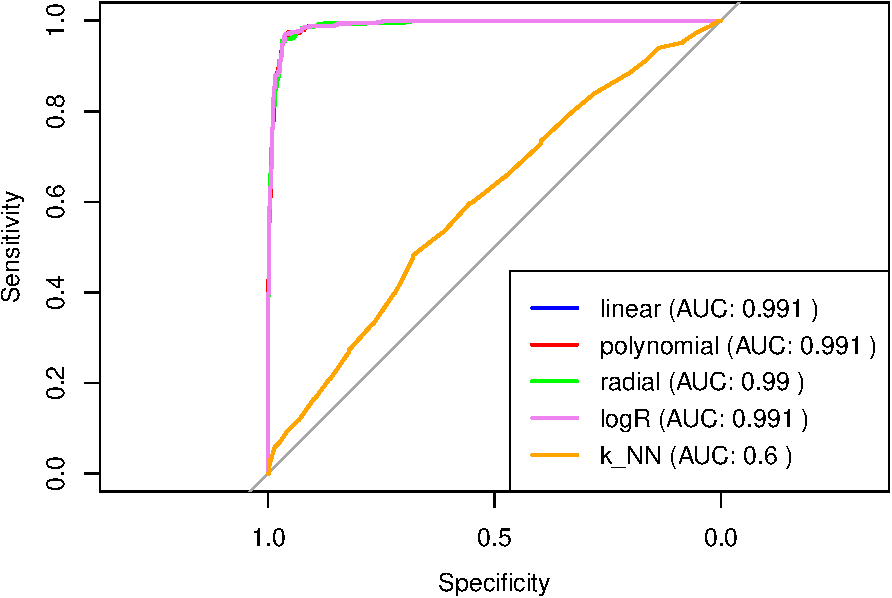
\includegraphics{Ergebnisse_files/figure-latex/S1ROC-1.pdf}
\caption{ROC-Kurven Szenario 1}
\label{fig:S1ROC}
\end{minipage}
\hfill
\begin{minipage}{0.48\linewidth}
\centering
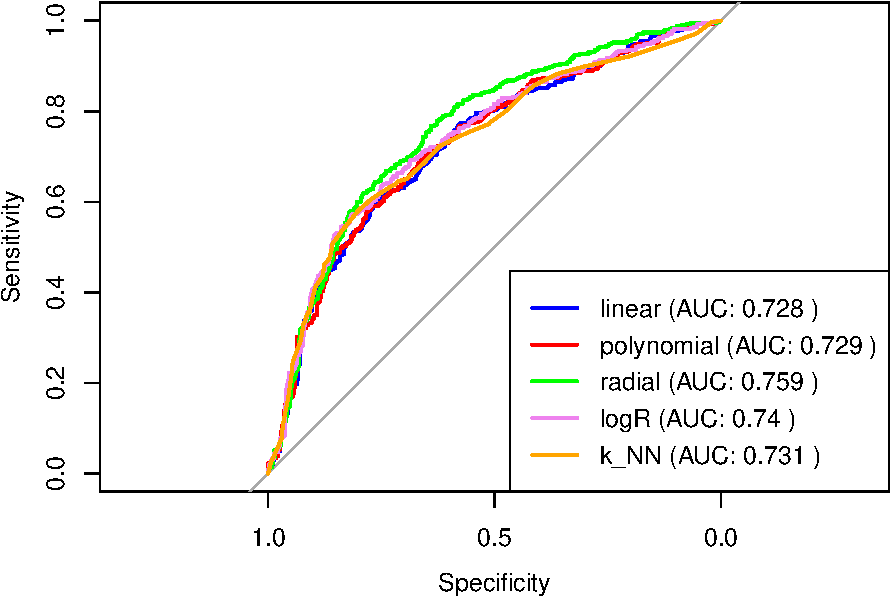
\includegraphics{Ergebnisse_files/figure-latex/S2ROC-1.pdf}
\caption{ROC-Kurven Szenario 2}
\label{fig:S2ROC}
\end{minipage}
\vspace*{0.5cm}\newline
\begin{minipage}{\linewidth}
\centering
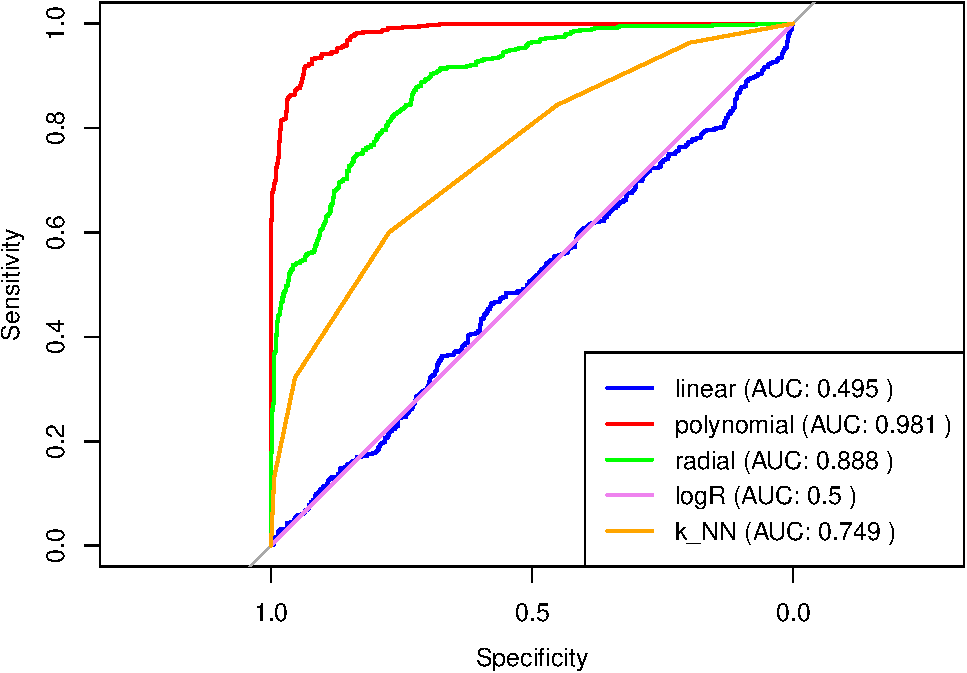
\includegraphics[width=0.48\linewidth]{Ergebnisse_files/figure-latex/S3ROC-1.pdf}
\caption{ROC-Kurven Szenario 3}
\label{fig:S3ROC}
\end{minipage}
\end{figure}

Abbildung \ref{fig:S3ROC} zeigt die ROC-Kurven für Szenario 3. Hieraus
wird deutlich, dass die Kurve von \textit{SVM-P} nahe an der oberen,
linken Ecke verläuft, was für eine nahezu perfekte Klassifikation
spricht. Der etwas flachere Verlauf von \textit{SVM-R} und \textit{K-NN}
macht deutlich, dass diese beiden Algorithmen weniger gute Leistung
zeigen. Dennoch können die beiden oben erwähnten Gruppen gut
identifiziert werden, da sich \textit{SVM-L} und \textit{LogR} nahe der
diagonalen Linie orientieren. Diese beschreibt eine ROC-Kurve einer
reinen Zufallsauswahl, woraus gefolgert werden kann, dass sie kaum
Fähigkeit aufweisen zwischen den Klassen zu unterscheiden. Diese
Szenarien bestätigen die Vermutung aus \textbf{H2} zwar nicht direkt, da
hier im Ranking über alle Szenarien mir radialer Entscheidungsgrenze
hinweg interessanterweise \textit{SVM-P} am besten performt aber
zumindest liegt hier \textit{SVM-R} auf dem zweiten Platz. Trotzdem
müssen wir mit diesen Ergebnissen \textbf{H2} ablehnen.

Zuletzt wird ein Vergleich der einzelnen Dimensionierungen über die drei
Formen der Entscheidungsgrenze gezogen. So ist für \(p \ll n\)
ersichtlich, dass insbesondere \textit{SVM-P} und \textit{SVM-R} über
alle drei Szenarien gute Leistung (mit Werten mindestens nahe 0.8)
erzielen. Auch im durchschnittlichen Ranking über alle drei Szenarien
hinweg zeigen die \textit{SVM}-Methoden die besten Ergebnisse.
Überaschen ist nur die unerwartet schlechte Performance von
\textit{K-NN}. Somit bestätigt sich \textbf{H3} hier nur teilweise. In
den hochdimensionalen Szenarien \(p \gg n\) ist einzig \textit{K-NN}
überzeugend, welcher auch im polynomialen Szenario Werte über 0.7
aufweist. Hier belegen die \textit{SVM}-Methoden tatsächlich sogar die
letzten Plätze im durchschnittlichen Ranking. Dies deutet klar darauf
hin, dass \textbf{H4} mit unseren Daten verworfen werden muss.

\section{Fazit}

In unserer Arbeit haben wir zum einen die Funktionsweise der Support
Vector Machines als binäre Klassifikationsmethode beleuchtet, als auch
die Leistungsfähigkeit in Datenszenarien mit verschiedenen Eigenschaften
verglichen. Diese Datensszenarien, wurden synthetisch von uns
hergestellt und sind in ihrem datengenerierenden Prozess speziell auf
\textit{SVM} zugeschnitten. Anschließend haben wir uns mit einschlägiger
Literatur beschäftigt, bei der die Autoren bereits ähnliche Versuche
durchgeführt haben und anhand dessen Hypothesen abgeleitet. Für die
Durchführung unserer Versuche haben wir die Performance von \textit{SVM}
mit verschiedenen Kernels sowie weiterer Klassifikationsmethoden über
alle Szenarien mit verschiedenen Maßzahlen verglichen. \newline 
Insgesamt mussten wir allerdings festellen, dass unsere Ergebnisse die
Hypothesen nur in Teilen bestätigen. \textit{SVM}-Methoden, haben im
Durschnitt oft bessere Leistungen gezeigt, als die anderen Methoden. Wir
schließen aufgrund der Rankings, dass, egal welche Dimensionierung
vorliegt und wenn keine Information über die Form der
Entscheidungsgrenze vorliegt, \textit{SVM} mit radialen und polynomialen
Kernel immer eine gute Entscheidung darstellen. Zumindest sollten diese
beiden dem \textit{SVM} mit linearem Kernel vorgezogen werden. Wobei
hier auch anzumerken ist, dass mit der höheren Flexibilität der
\textit{SVM-P} und \textit{SVM-R} auch die Gefahr besteht, dass es zu
Overfitting kommt. Dies könnte vor allem bei empirischen Daten zu
höheren Klassifikationsfehlern führen.\newline Allerdings haben wider
Erwarten die \text{SVM} mit dem Kernel der auf die Datenerzeugung
eigentlich zugeschnitten ist nicht besser performt. Wir vermuten, dass
es an einem zu niedrigen \(n\)-Wert in der Dimensionierung für die
Szenarien 4 bis 9 liegen könnte und dass sich in einer etwaigen
Simulationsstudie mit dem gleichen DGP und Dimensionierung die Hypothese
vielleicht doch noch bestätigen könnte, da sich so zufällige
Abweichungen aufheben. Was das Verhalten in den verschiedenen
Dimensionalitäten angeht können wir zumindest sagen, dass in Fällen mit
mehr Beobachtungen als Variablen \textit{SVM} eine gute Wahl darstellen.
Schwieriger wird es bei den hochdimensionalen Szenarien, da hier
\textit{K-NN} eindeutig besser performt hat. Uns fällt es schwer dies zu
erklären, da wir eigentlich davon ausgingen, dass \textit{K-NN} bei
vielen Variablen eher schlechter performt.

Wir sehen daher Optimierungsmöglichkeiten für weitere Arbeiten dieser
Art. So wäre es angebracht, wie bereits erwähnt die Datengererierung für
die einzelnen Szenarien wiederholt durchzuführen und die Ergebnisse zu
mitteln. Die Dimesnionierung könnte auch so angepasst werden, dass die
\(n\) Werte etwas höher sind auch für Szenarien mit \(p \gg n\).\\
Des Weiteren könnte der Einfluss der Szenarien auf die Berechnungszeit
für die \textit{SVM}-Algorithmen noch einbezogen werden. Ein
Benchmark-Test könnte auch hier zu interessanten Ergebnissen führen.
Zusätzlich haben wir hier lediglich eine handvoll
Klassifikationsalgorithmen im Vergleich untersucht. Eine Erweiterung auf
\textit{Classification Trees}, \textit{Discriminant Analysis} oder
verschiedene \textit{Ensemble-Methoden} ist denkbar. An der
Datengenerierung ließen sich ebenfalls weitere Aspekte anpassen. So
könnte die Anteile der Ausprägungen in der binären Zielvariable noch
variiert, mehr als zwei Ausprägungen generiert oder auch komplexere
Entscheidungsgrenzen modelliert werden. Diese Erweiterungen hätten
allerdings den Rahmen dieser Arbeit überschritten. Trotzdem ergänzt
unsere Arbeit die bisherigen Befunde zur Leistungs- und
Anpassungsfähigkeit von Support-Vector Machines in verschiedenen
Datensituation, sowie deren Bedeutung im Kontext von
Klassifikationsaufgaben. \newpage

\addcontentsline{toc}{section}{Literatur}

\printbibliography

\end{document}
